\documentclass{ws-ijbc}

%%%%%%%%%%%%%%%%
% Instructions %
%%%%%%%%%%%%%%%%
% Set the document class and settings to match the final document that these figures will be included into
% This will output a pdf with a page for each figure, nicely cropped according to picture dimenstions as defined below in the `Figure' Section. Inlcude in the final document by using package 'graphicx' and command \includegraphics[page=<page of figure>]{figures.pdf}
% The following package is used to create the cropping mentioned above, and apparently should be the last loaded package: \usepackage[active,tightpage]{preview}
% The following command re-writes the figure enviroment to become a preview enviroment - without this spacing is off, and captions and labels may appear
%\renewenvironment{figure}[1][]{%
%	\begin{preview}%
%		\renewcommand{\caption}[2][]{}}
%	{\end{preview}}

%%%%%%%%%%%%%%%%%
% Load Packages %
%%%%%%%%%%%%%%%%%
\usepackage{epsfig}
\usepackage{amssymb}
\pagestyle{empty}
\usepackage{epstopdf}
\usepackage{mathrsfs}
\usepackage{amsmath}
\usepackage{graphicx}
\usepackage{array}
\usepackage{xcolor}    % \nopagecolor
\usepackage{fp}
\usepackage{bm}    % boldmath \bm{}
\usepackage[pdftex,active,tightpage]{preview}    % should be loaded lasts
% adjust borders added to figures: left, lower, right and upper borders. - useful to increase lower border not to cut off labels placed below figure bounds. 
\renewcommand{\PreviewBbAdjust}{0mm -0.25mm 0mm 0mm}
\renewenvironment{figure}[1][]{%
	\begin{preview}%
		\renewcommand{\caption}[2][]{}}
	{\end{preview}}

\setlength{\unitlength}{1cm}

%%%%%%%%%%%%%%%%%%%%%%%%%%%%%%%%%%%%%%%%%%%%%%%%
% Get various dimensions for the documentclass %
%%%%%%%%%%%%%%%%%%%%%%%%%%%%%%%%%%%%%%%%%%%%%%%%
\makeatletter
\newcommand*{\getlength}[1]{\strip@pt\dimexpr0.035136\dimexpr#1\relax\relax}
\newcommand{\showfont}{%
encoding: \f@encoding{},\\
family: \f@family{},\\
series: \f@series{},\\
shape: \f@shape{},\\
size: \f@size{} pt,\\
text height: \getlength{\the\textheight} cm,\\
text width:     \getlength{\the\textwidth} cm}
\makeatother

%\begin{document}
%\begin{figure}
%	\begin{picture}(20,5)(0,0)
%		\showfont
%	\end{picture}
%\end{figure}
%\newpage
%%%%%%%%%%%%%%%%
%%% Critical manifold %%%
%%%%%%%%%%%%%%%%
\nopagecolor
\begin{figure}
	\begin{picture}(9,5)(0,0)
	\put(0.74,0.74){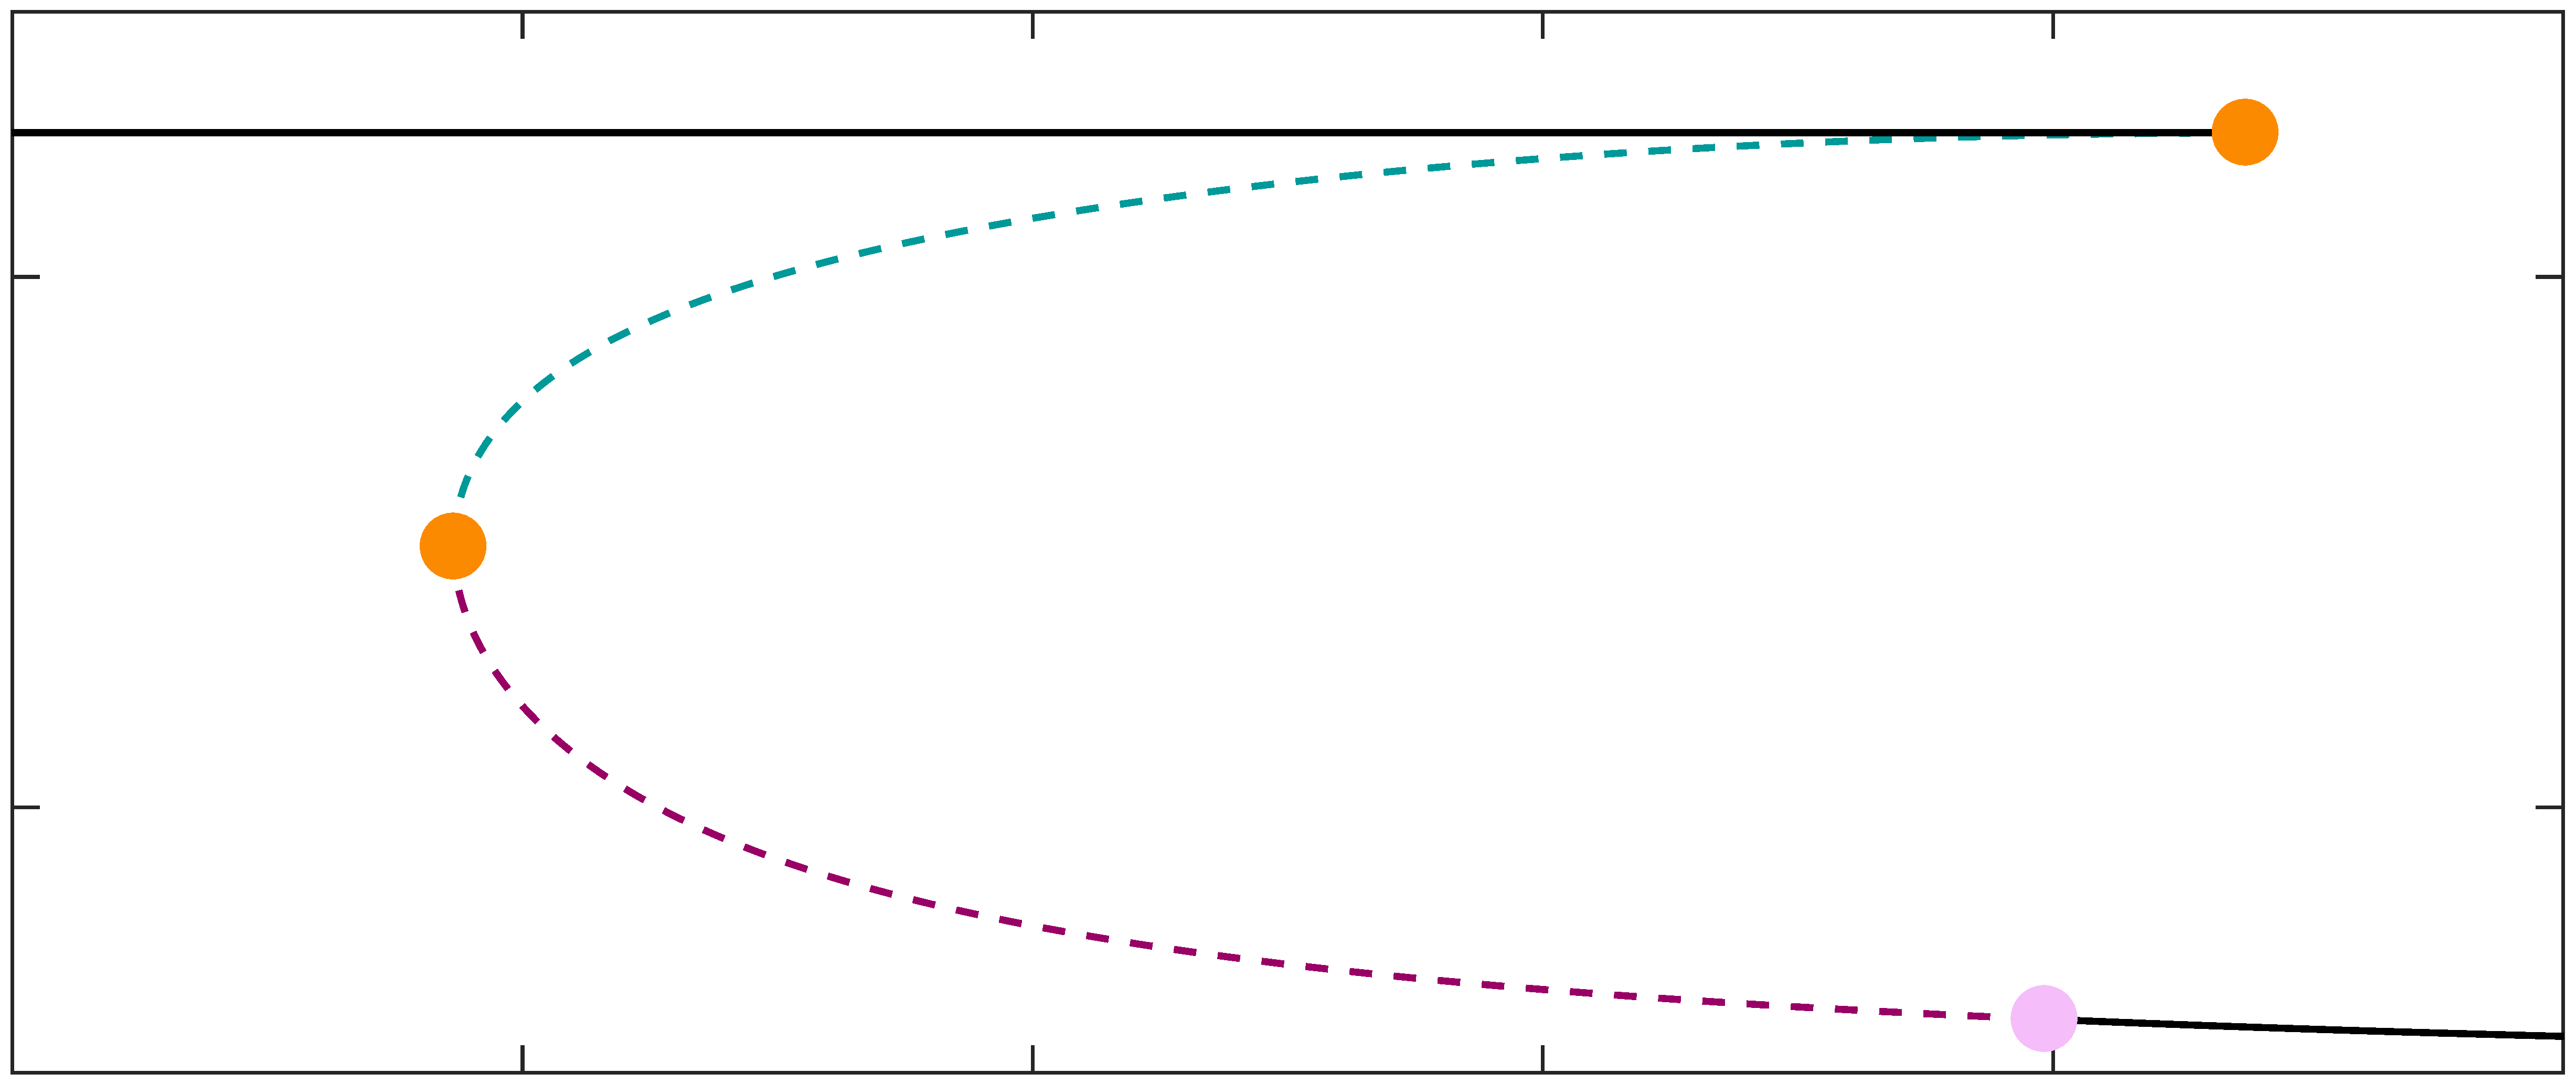
\includegraphics[width=8cm,height=4cm]{./figures/paper_critical.eps}}
	\put(7.9,4.12){$F_1$}
        \put(1.55,2.65){$F_2$}
        \put(7,1.2){$H$}
        \put(4.4,3.65){$C^t$}
        \put(4.4,1.35){$C^b$}
        \put(0.5,4.5){$A$}
        \put(0.2,3.65){$9.0$}
        \put(0.2,1.65){$3.0$}
	\put(2.12,0.35){$0.3$}
	\put(3.72,0.35){$0.5$}
	\put(5.32,0.35){$0.7$}
	\put(6.92,0.35){$0.9$}
	\put(8.4,0.45){$B$}
	\put(2.1,1.75){$\chi$}
	\end{picture}
	\caption{}
\end{figure}
\newpage

%%%%%%%%%%%%%%%%
%%% Tube figure %%%
%%%%%%%%%%%%%%%%

\begin{figure}
	\begin{picture}(16,9)(0,0)
	    \put(0.75,0.75){\includegraphics[width=15cm, height=8cm]{./figures/paper_slow.eps}}
	    \put(14.1,7.97){$F_1$}
	    \put(9.85,6.5){$D_\delta(B_{\mathrm{out}})$}
	    \put(4,2.85){$D_\delta(B_{\mathrm{in}})$}
	    \put(7.0,5.97){$S^t$}
	    \put(0.45,8.47){$A$}
	    \put(0.0,2.65){7.25}
	    \put(0.0,6.6){9.75}
            \put(15.45,0.45){$B$}
            \put(3.52,0.35){$0.3$}
            \put(6.5,0.35){$0.5$}
            \put(9.51,0.35){$0.7$}
            \put(12.5,0.35){$0.9$}
	\end{picture}
	\caption{}
\end{figure}

\newpage
%%%%%%%%%%%%%%%%
%%% Step 1 %%%
%%%%%%%%%%%%%%%%

\begin{figure}
	\begin{picture}(9,5)(0.0,0.0)
	\put(0.75,0.75){\includegraphics[width=8cm, height=4cm]{./figures/step1.eps}}
	\put(7.9,4.1){$F_1$}
        \put(1.55,2.68){$F_2$}
        \put(7,3.5){$E^s(p^t_{\mathrm{out}})$}
        \put(6.95,1.25){$H$}
        \put(1.4,3.85){$\Sigma^*$}
        \put(4.5,3.35){$S^t$}
        \put(2.15,0.35){$0.3$}
        \put(3.73,0.35){$0.5$}
        \put(5.3,0.35){$0.7$}
        \put(6.85,0.35){$0.9$}
        \put(0.25,1.6){$3.0$}
        \put(0.25,3.6){$9.0$}
        \put(0.5,4.45){$A$}
        \put(8.4,0.47){$B$}
        \put(2.2,1.68){$\chi$}

	\end{picture}
	\caption{}
\end{figure}

\newpage
%%%%%%%%%%%%%%%%
%%% Step 2 %%%
%%%%%%%%%%%%%%%%

\begin{figure}
	\begin{picture}(9,5)(0.0,0.0)
	\put(0.75,0.75){\includegraphics[width=8cm, height=4cm]{./figures/step2.eps}}
	\put(7.9,4.1){$F_1$}
        \put(1.55,2.68){$F_2$}
        \put(7,3.5){$E^s(p^t_{\mathrm{out}})$}
        \put(6.95,1.25){$H$}
        \put(1.4,3.85){$\Sigma^*$}
        \put(4.5,3.35){$S^t$}
        \put(2.15,0.35){$0.3$}
        \put(3.73,0.35){$0.5$}
        \put(5.3,0.35){$0.7$}
        \put(6.85,0.35){$0.9$}
        \put(0.25,1.6){$3.0$}
        \put(0.25,3.6){$9.0$}
        \put(0.5,4.45){$A$}
        \put(8.4,0.47){$B$}

	\end{picture}
	\caption{}
\end{figure}


\newpage
%%%%%%%%%%%%%%%%
%%% Step 3 %%%
%%%%%%%%%%%%%%%%

\begin{figure}
	\begin{picture}(9,5)(0.0,0.0)
	\put(0.75,0.75){\includegraphics[width=8cm, height=4cm]{./figures/step3.eps}}
	\put(7.9,4.1){$F_1$}
        \put(1.55,2.68){$F_2$}
        \put(6.9,3.4){$\Omega$}
        \put(6.95,1.25){$H$}
        \put(1.5,3.55){$\psi$}
        \put(4.5,3.35){$S^t$}
        \put(2.15,0.35){$0.3$}
        \put(3.73,0.35){$0.5$}
        \put(5.3,0.35){$0.7$}
        \put(6.85,0.35){$0.9$}
        \put(0.25,1.6){$3.0$}
        \put(0.25,3.6){$9.0$}
        \put(0.5,4.45){$A$}
        \put(8.4,0.47){$B$}

	\end{picture}
	\caption{}
\end{figure}


\newpage
%%%%%%%%%%%%%%%%
%%% Step 4 %%%
%%%%%%%%%%%%%%%%

\begin{figure}
	\begin{picture}(9,5)(0.0,0.0)
	\put(0.75,0.75){\includegraphics[width=8cm, height=4cm]{./figures/step4.eps}}
	\put(7.9,4.1){$F_1$}
        \put(1.55,2.68){$F_2$}
        \put(6.9,3.4){$\Omega$}
        \put(6.95,1.25){$H$}
        \put(3,1.75){$\psi$}
        \put(4.5,3.35){$S^t$}
        \put(2.15,0.35){$0.3$}
        \put(3.73,0.35){$0.5$}
        \put(5.3,0.35){$0.7$}
        \put(6.85,0.35){$0.9$}
        \put(0.25,1.6){$3.0$}
        \put(0.25,3.6){$9.0$}
        \put(0.5,4.45){$A$}
        \put(8.4,0.47){$B$}

	\end{picture}
	\caption{}
\end{figure}


\newpage

%%%%%%%%%%%%%%%%
%% One submanifold BAX %%
%%%%%%%%%%%%%%%%

\begin{figure}
	\begin{picture}(18,12.5)(0,0)
        	\put(17,11.5){$\text{(a)}$}
	\put(0,0){\includegraphics[width=18cm, height=12.5cm]{./figures/one_piece_BAX.png}}
		
	\end{picture}
	\caption{}
\end{figure}

\newpage
%%%%%%%%%%%%%%%%
%% One submanifold BAY %%
%%%%%%%%%%%%%%%%

\begin{figure}
	\begin{picture}(18,12.5)(0,0)
		\put(17,11.5){$\text{(b)}$}
	    \put(0,0){\includegraphics[width=18cm, height=12.5cm]{./figures/one_piece_BAY.png}}
	\end{picture}
	\caption{}
\end{figure}

\newpage
%%%%%%%%%%%%%%%%
%%% Pieces BAX %%%
%%%%%%%%%%%%%%%%

\begin{figure}
	\begin{picture}(18,12.5)(0,0)
	    \put(0,0){\includegraphics[width=18cm, height=12.5cm]{./figures/paper_pieces_BAX.eps}}
	    \put(17,11.5){$\text{(a)}$}
	\end{picture}
	\caption{}
\end{figure}

\newpage
%%%%%%%%%%%%%%%%
%%% Pieces BAY %%%
%%%%%%%%%%%%%%%%

\begin{figure}
	\begin{picture}(18,12.5)(0,0)
	    \put(0,0){\includegraphics[width=18cm, height=12.5cm]{./figures/paper_pieces_BAY.eps}}
	    \put(17,11.5){$\text{(b)}$}
	\end{picture}
	\caption{}
\end{figure}

\newpage
%%%%%%%%%%%%%%%%
%%% Lin 1 %%%
%%%%%%%%%%%%%%%%

\begin{figure}
	\begin{picture}(9,5)(0,0)
	   	\put(0.75,0.75){\includegraphics[width=8cm, height=4cm]{./figures/Lin1.eps}}
	    	\put(4.5,3.35){$S^t$}
		\put(4.5,1.6){$S^b$}
        		\put(2.15,0.35){$0.3$}
        		\put(3.73,0.35){$0.5$}
        		\put(5.3,0.35){$0.7$}
        		\put(6.85,0.35){$0.9$}
        		\put(0.25,1.6){$3.0$}
        		\put(0.25,3.6){$9.0$}
        		\put(0.5,4.45){$A$}
        		\put(8.4,0.47){$B$}
	\end{picture}
	\caption{}
\end{figure}

\newpage
%%%%%%%%%%%%%%%%
%%% Lin 2 %%%
%%%%%%%%%%%%%%%%


\begin{figure}
	\begin{picture}(9,5)(0,0)
	    \put(0.75,0.75){\includegraphics[width=8cm, height=4cm]{./figures/Lin2.eps}}
	        \put(2.15,0.35){$0.3$}
        		\put(3.73,0.35){$0.5$}
        		\put(5.3,0.35){$0.7$}
        		\put(6.85,0.35){$0.9$}
        		\put(0.25,1.6){$3.0$}
        		\put(0.25,3.6){$9.0$}
        		\put(0.5,4.45){$A$}
        		\put(8.4,0.47){$B$}
	\end{picture}
	\caption{}
\end{figure}

\newpage

%%%%%%%%%%%%%%%%
%%% Lin 3 %%%
%%%%%%%%%%%%%%%%


\begin{figure}
	\begin{picture}(9,5)(0,0)
	    \put(0.75,0.75){\includegraphics[width=8cm, height=4cm]{./figures/Lin3.eps}}        		
	     \put(2.15,0.35){$0.3$}
        	      \put(3.73,0.35){$0.5$}
        		\put(5.3,0.35){$0.7$}
        		\put(6.85,0.35){$0.9$}
        		\put(0.25,1.6){$3.0$}
        		\put(0.25,3.6){$9.0$}
        		\put(0.5,4.45){$A$}
        		\put(8.4,0.47){$B$}
	\end{picture}
	\caption{}
\end{figure}

\newpage

%%%%%%%%%%%%%%%%
%%% Lin 3 %%%
%%%%%%%%%%%%%%%%


\begin{figure}
	\begin{picture}(9,5)(0,0)
	    \put(0.75,0.75){\includegraphics[width=8cm, height=4cm]{./figures/Lin4.eps}}
	        \put(2.15,0.35){$0.3$}
        		\put(3.73,0.35){$0.5$}
        		\put(5.3,0.35){$0.7$}
        		\put(6.85,0.35){$0.9$}
        		\put(0.25,1.6){$3.0$}
        		\put(0.25,3.6){$9.0$}
        		\put(0.5,4.45){$A$}
        		\put(8.4,0.47){$B$}

	   \end{picture}
	\caption{}
\end{figure}

\newpage

%%%%%%%%%%%%%%%%
%%% Figure %%%
%%%%%%%%%%%%%%%%


\begin{figure}
	\begin{picture}(19,13)(0,0)
	    \put(0,0){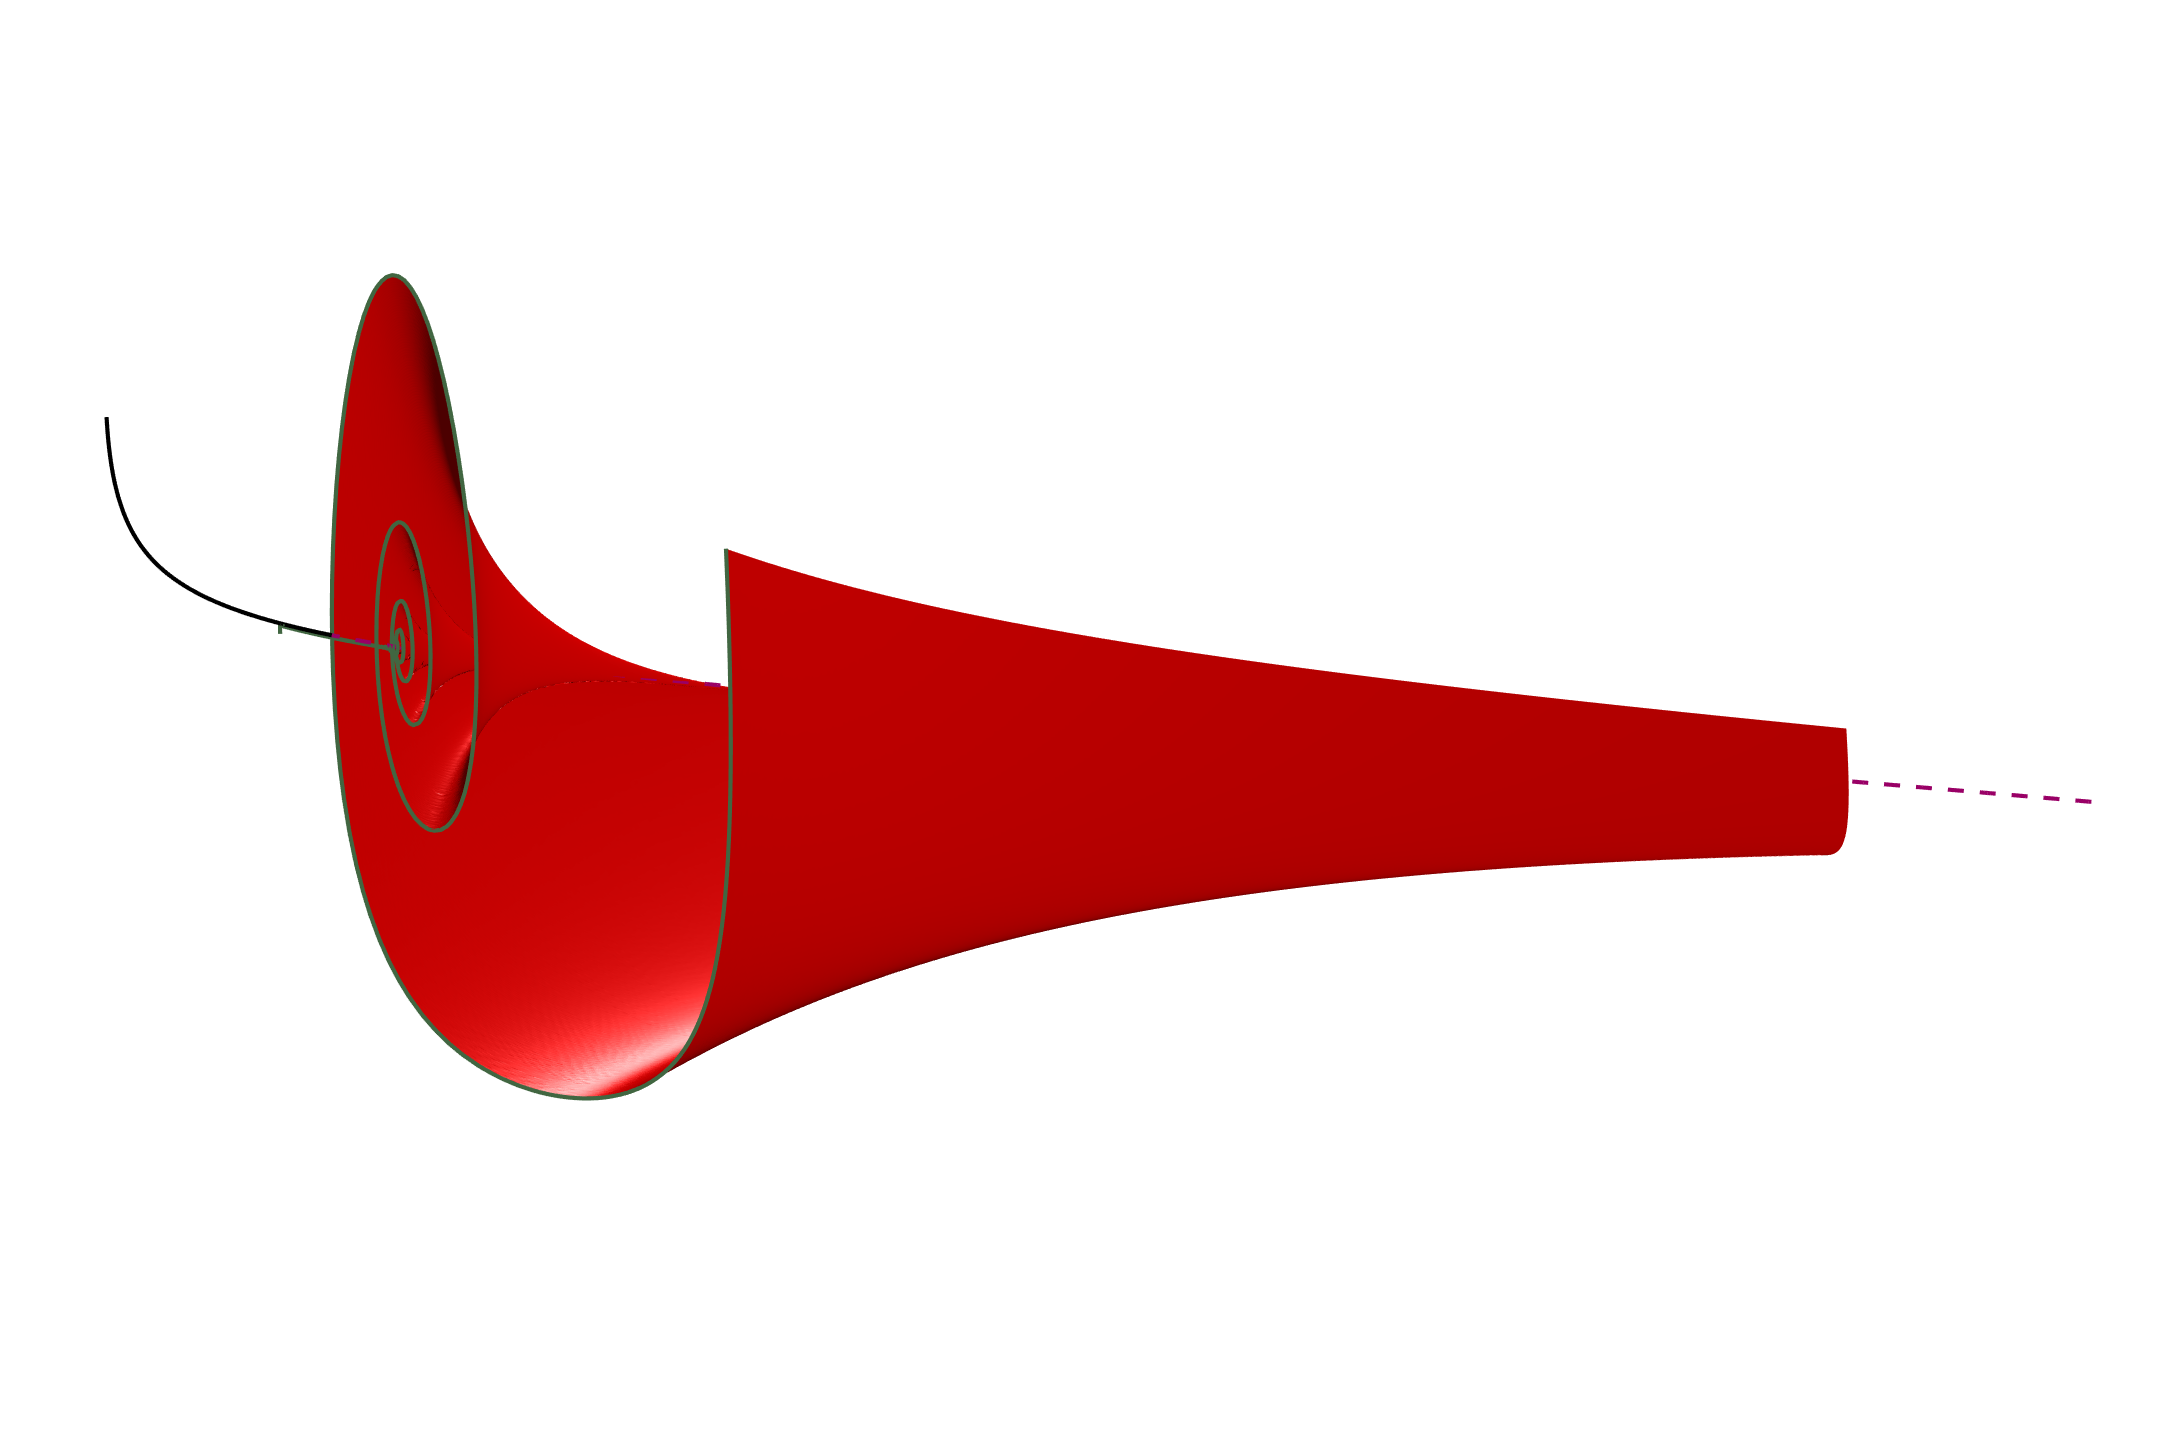
\includegraphics[width=\textwidth]{./figures/unstable_piece_BAX.eps}}
	\end{picture}
	\caption{}
\end{figure}

\newpage
%%%%%%%%%%%%%%%%
%%% Figure %%%
%%%%%%%%%%%%%%%%


\begin{figure}
	\begin{picture}(19,13)(0,0)
	    \put(0,0){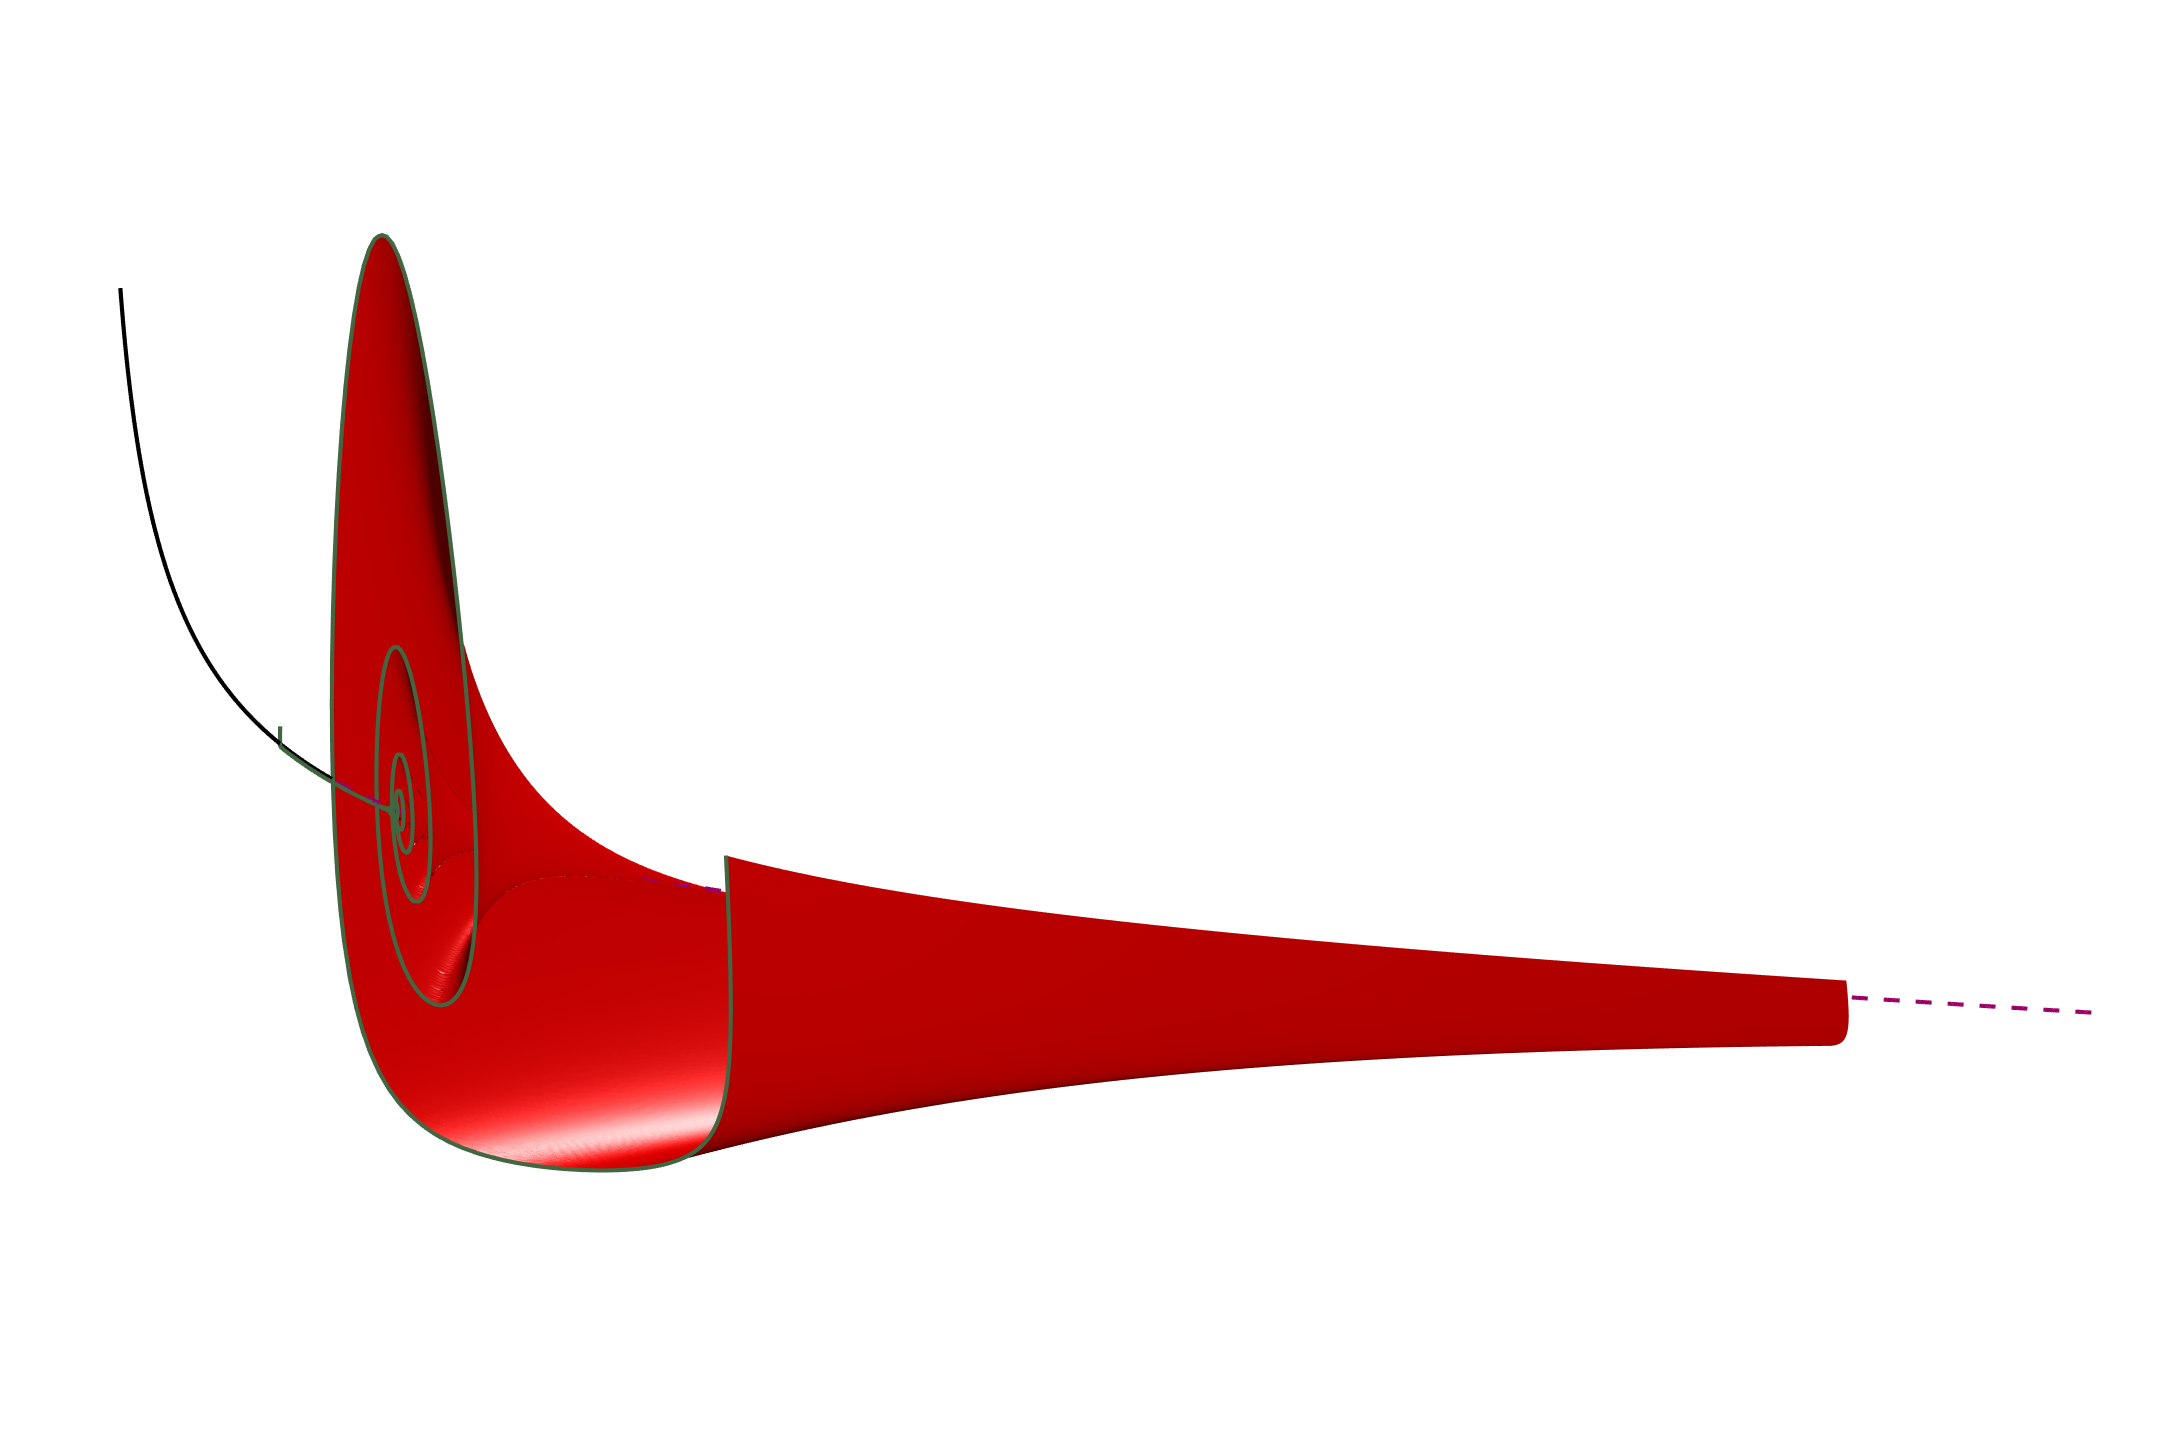
\includegraphics[width=\textwidth]{./figures/unstable_piece_BAY.eps}}
	\end{picture}
	\caption{}
\end{figure}

\newpage

%%%%%%%%%%%%%%%%
%% Two submanifold BAX %%
%%%%%%%%%%%%%%%%

\begin{figure}
	\begin{picture}(18,12.5)(0,0)
       
	\put(0,0){\includegraphics[width=18cm, height=12.5cm]{./figures/two_pieces_BAX.eps}}
	\put(17,11.5){$\text{(a)}$}	
	\end{picture}
	\caption{}
\end{figure}

\newpage
%%%%%%%%%%%%%%%%
%% Two submanifold BAY %%
%%%%%%%%%%%%%%%%

\begin{figure}
	\begin{picture}(18,12.5)(0,0)
			    \put(0,0){\includegraphics[width=18cm, height=12.5cm]{./figures/two_pieces_BAY.eps}}
        		\put(17,11.5){$\text{(b)}$}
	\end{picture}
	\caption{}
\end{figure}

\newpage

%%%%%%%%%%%%%%%%
%%% MMO %%%
%%%%%%%%%%%%%%%%


\begin{figure}6
	\begin{picture}(17,10)(0,0)
	    \put(0,0){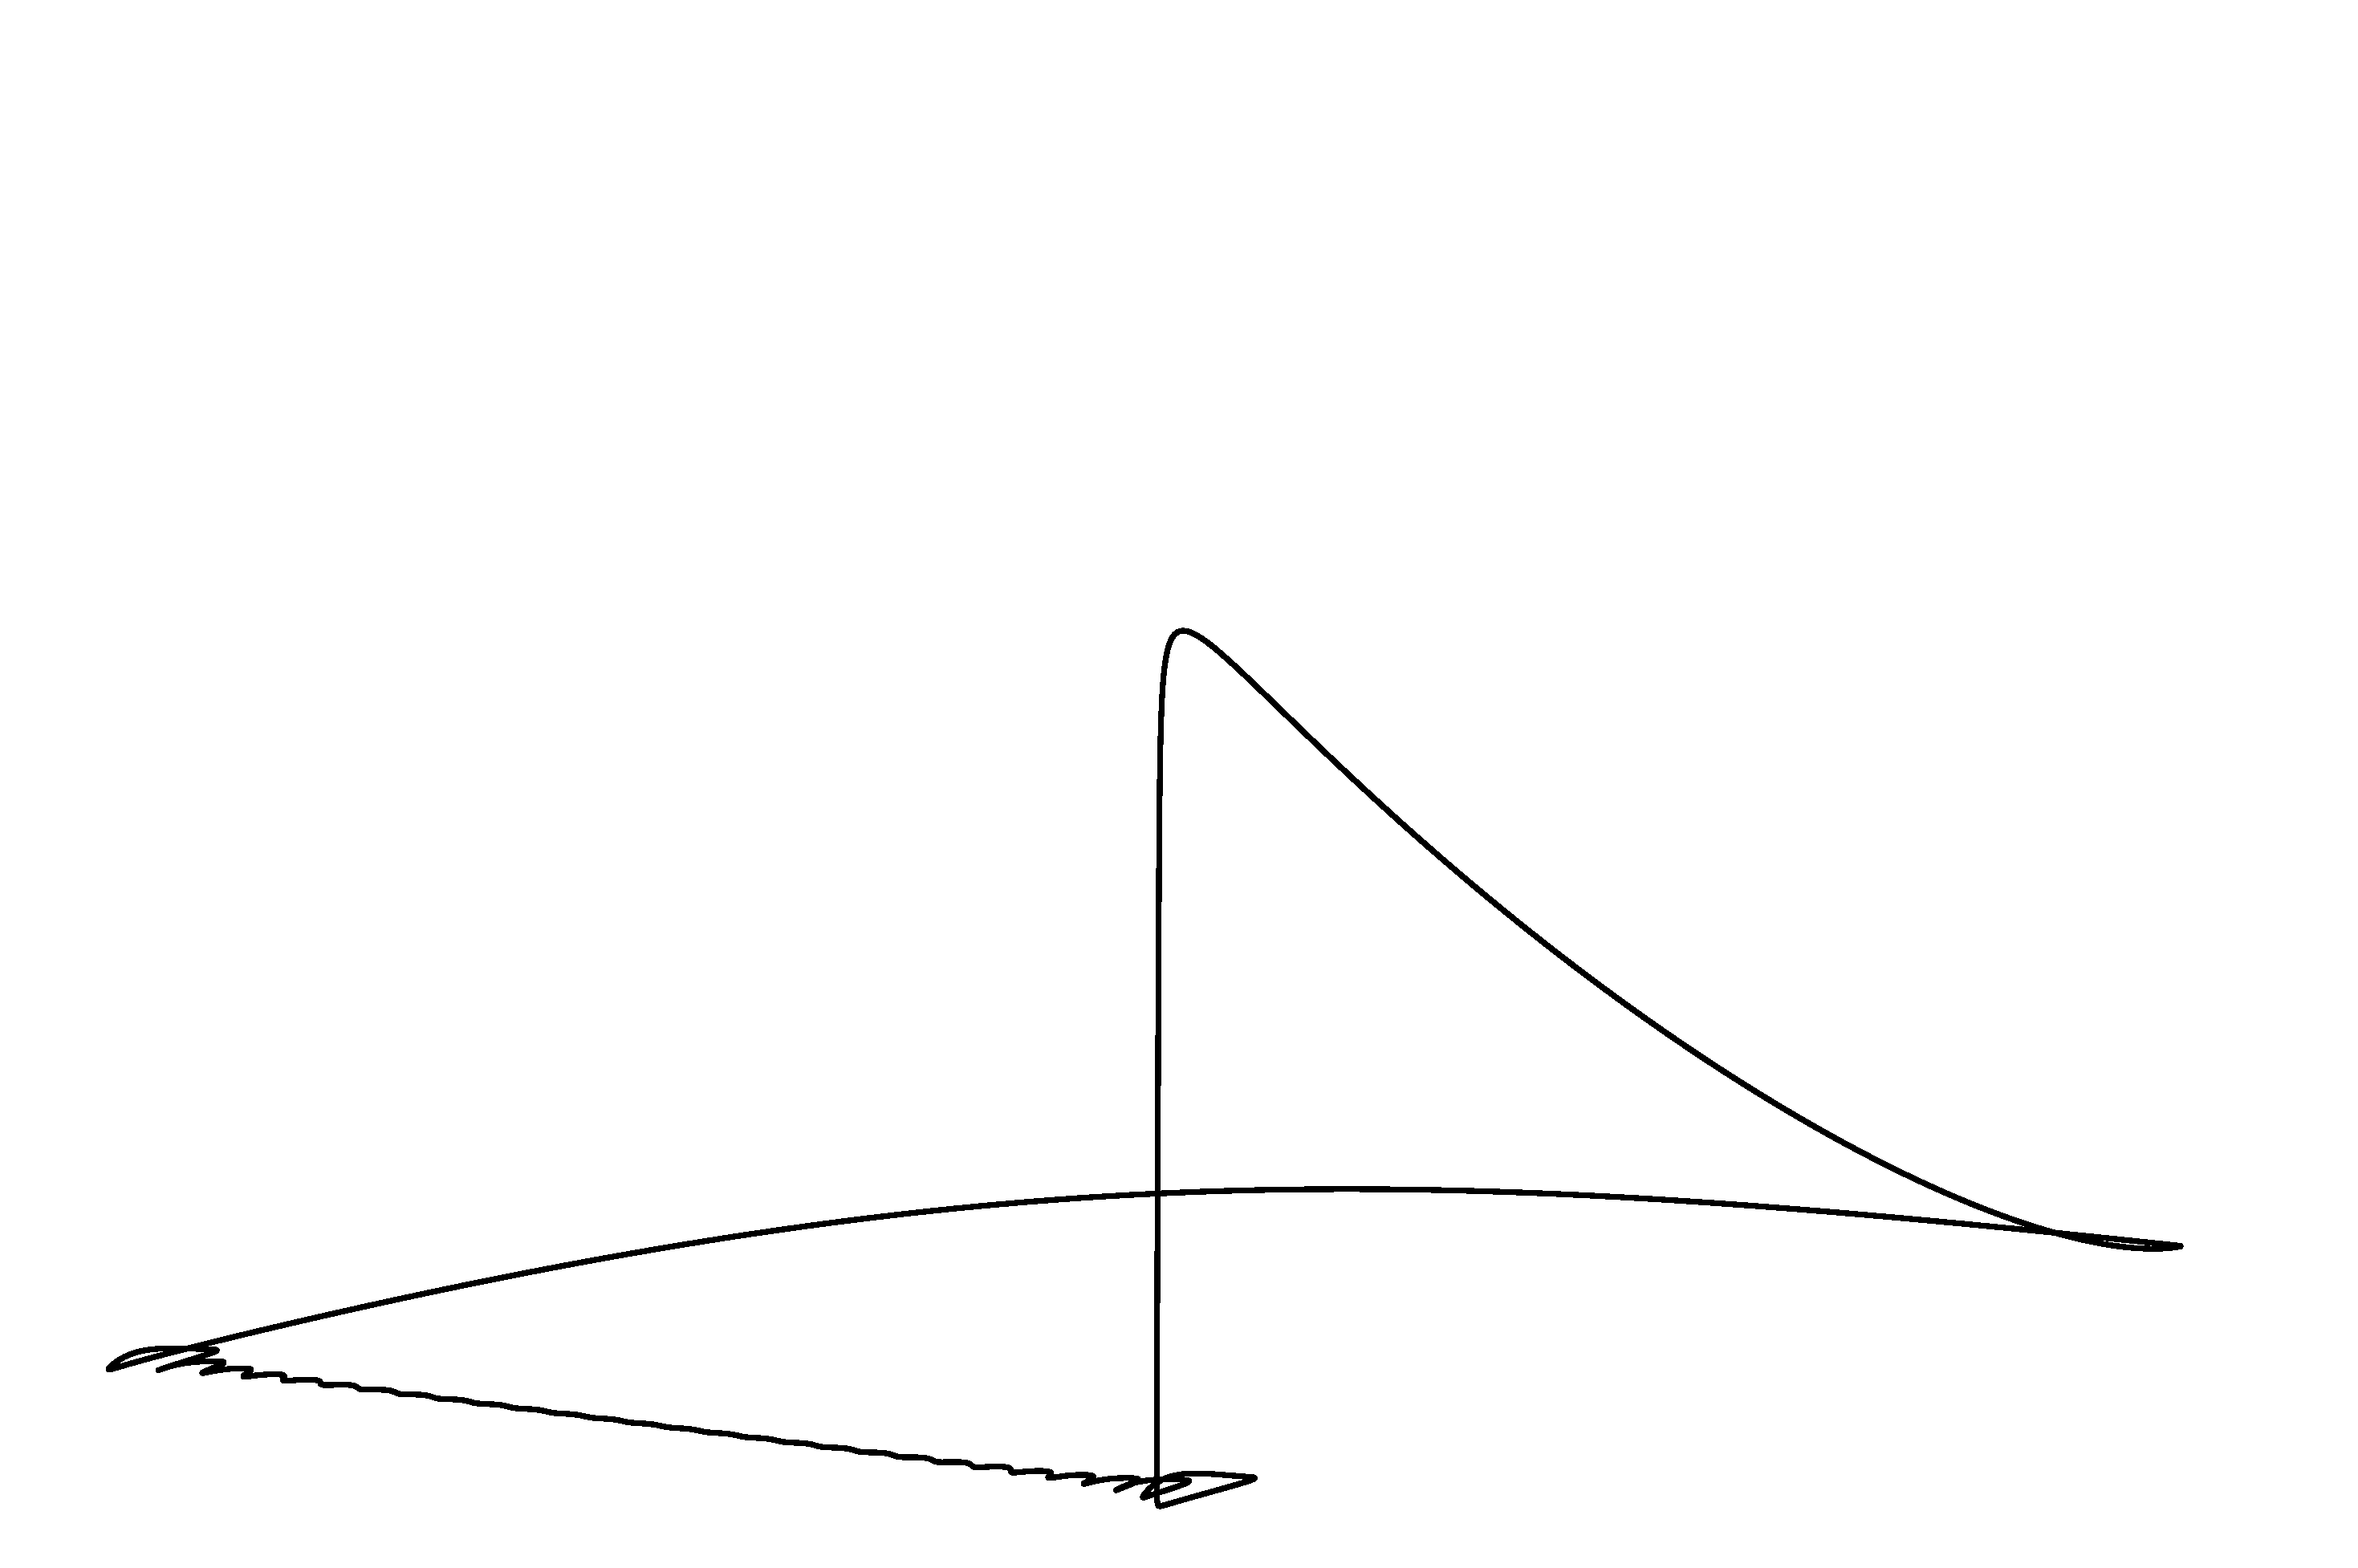
\includegraphics[width=\textwidth]{./figures/MMO_BAX.eps}}
	\end{picture}
	\caption{}
\end{figure}

\newpage

%%%%%%%%%%%%%%%%
%%% MMO %%%
%%%%%%%%%%%%%%%%

\begin{figure}
	\begin{picture}(16,10)(0,0)
	    \put(0,0){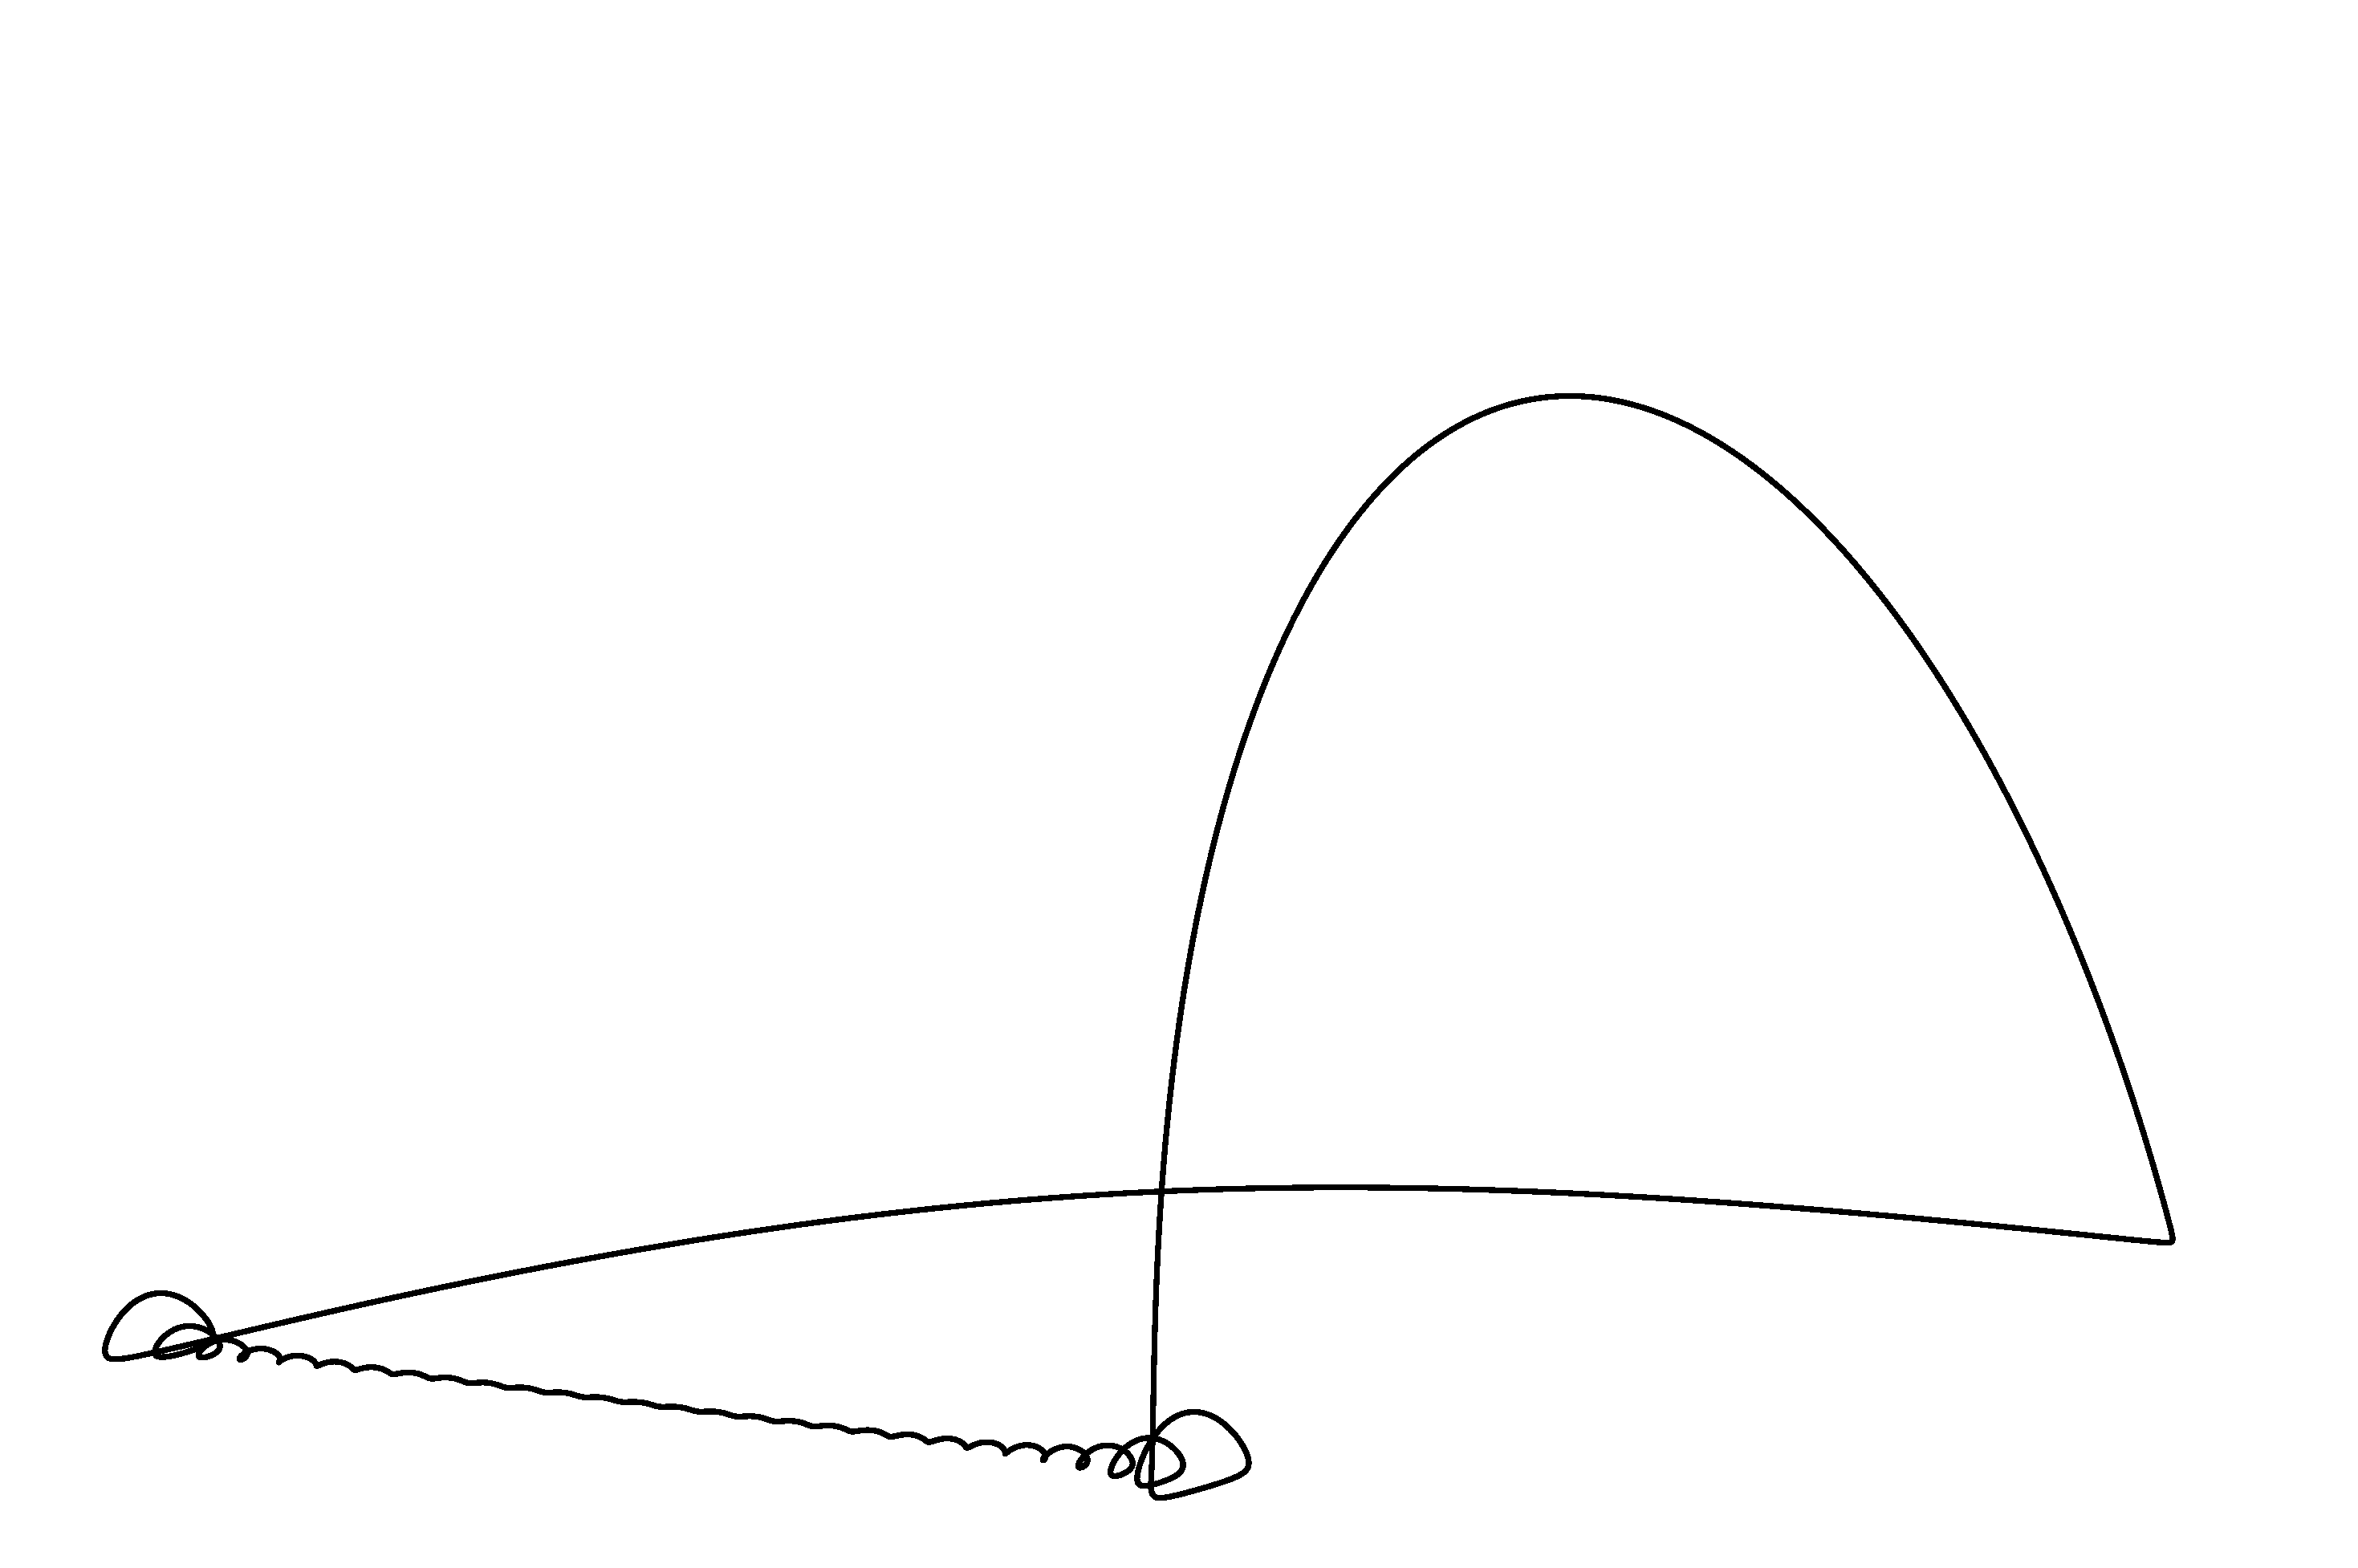
\includegraphics[width=\textwidth]{./figures/MMO_BAY.eps}}
	\end{picture}
	\caption{}
\end{figure}

\newpage

%%%%%%%%%%%%%%%%
%%% Figure %%%
%%%%%%%%%%%%%%%%

\begin{figure}
	\begin{picture}(19,13)(0,0)
	    \put(0,0){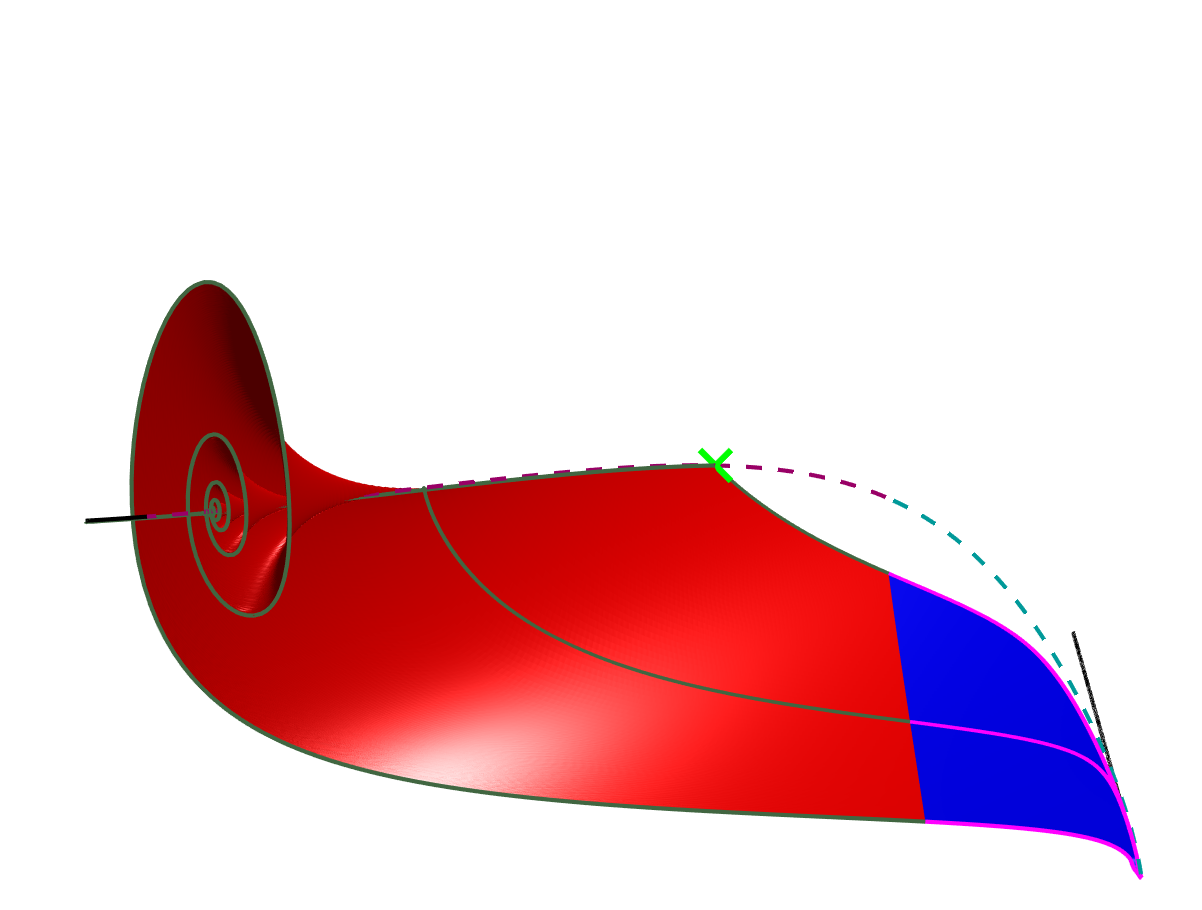
\includegraphics[width=\textwidth]{./figures/hetclin_6_BAX.eps}}
	\end{picture}
	\caption{}
\end{figure}

\newpage

%%%%%%%%%%%%%%%%
%%% Figure %%%
%%%%%%%%%%%%%%%%

\begin{figure}
	\begin{picture}(19,13)(0,0)
	    \put(0,0){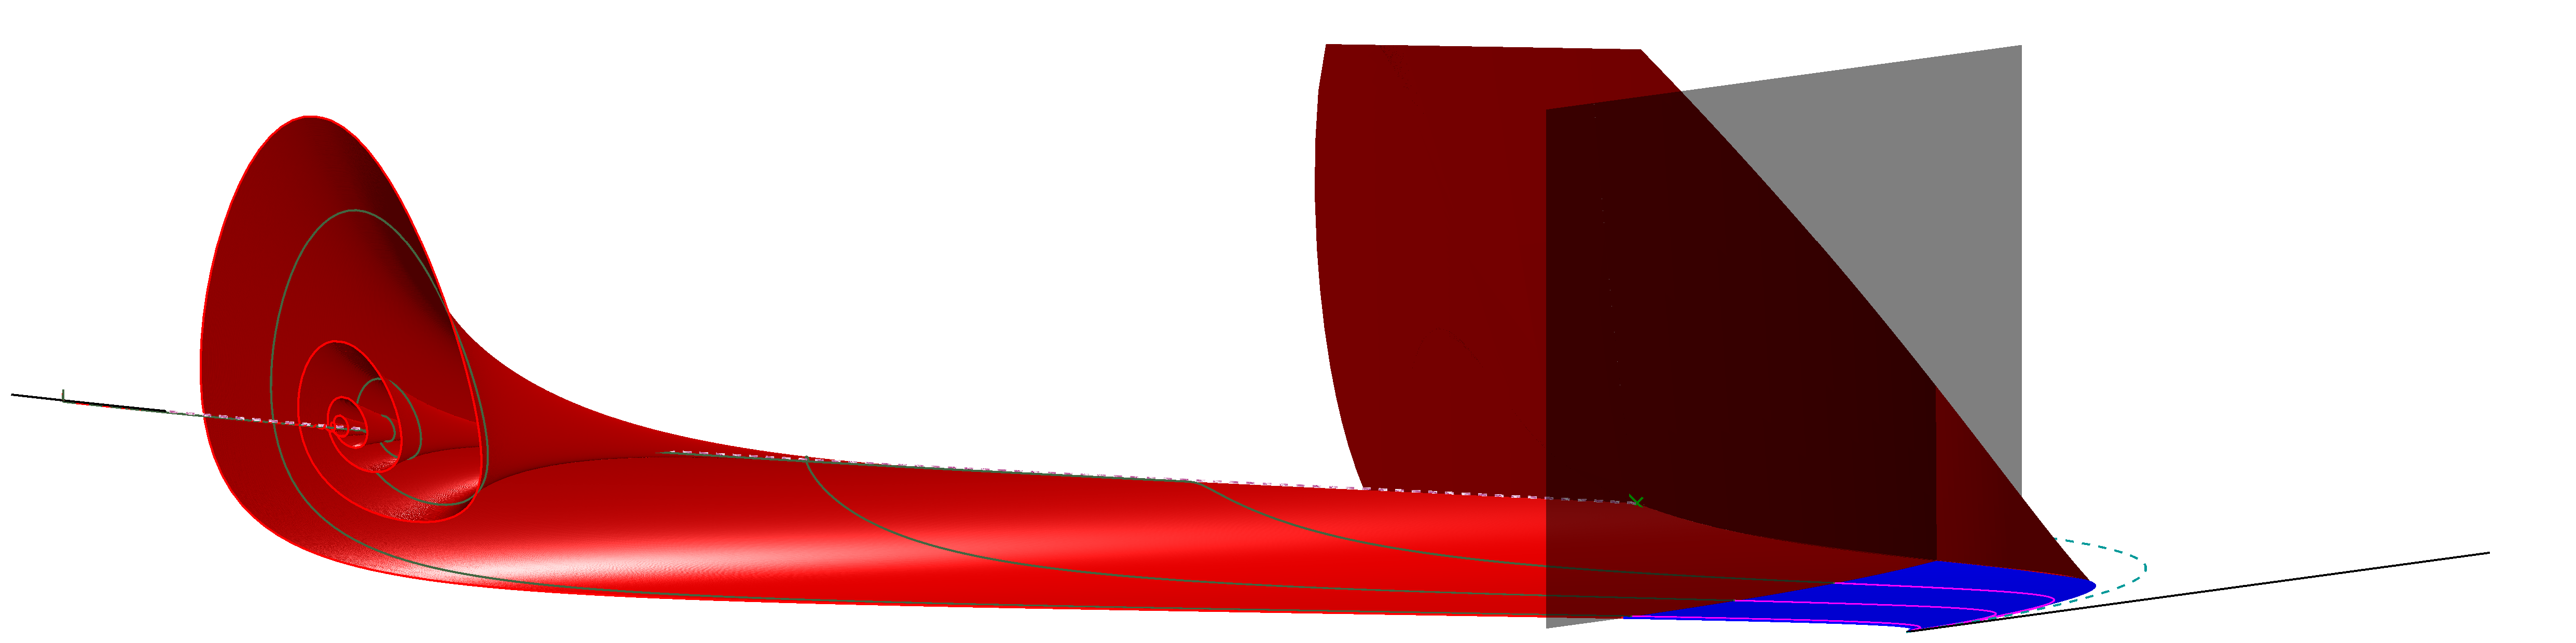
\includegraphics[width=\textwidth]{./figures/hetclin_6_BAY.eps}}
	\end{picture}
	\caption{}
\end{figure}

\newpage



\end{document}